\documentclass[a4paper]{book}
\usepackage{makeidx}
\usepackage{natbib}
\usepackage{graphicx}
\usepackage{multicol}
\usepackage{float}
\usepackage{listings}
\usepackage{color}
\usepackage{ifthen}
\usepackage[table]{xcolor}
\usepackage{textcomp}
\usepackage{alltt}
\usepackage{ifpdf}
\ifpdf
\usepackage[pdftex,
            pagebackref=true,
            colorlinks=true,
            linkcolor=blue,
            unicode
           ]{hyperref}
\else
\usepackage[ps2pdf,
            pagebackref=true,
            colorlinks=true,
            linkcolor=blue,
            unicode
           ]{hyperref}
\usepackage{pspicture}
\fi
\usepackage[utf8]{inputenc}
\usepackage{mathptmx}
\usepackage[scaled=.90]{helvet}
\usepackage{courier}
\usepackage{sectsty}
\usepackage[titles]{tocloft}
\usepackage{doxygen}
\lstset{language=C++,inputencoding=utf8,basicstyle=\footnotesize,breaklines=true,breakatwhitespace=true,tabsize=8,numbers=left }
\makeindex
\setcounter{tocdepth}{3}
\renewcommand{\footrulewidth}{0.4pt}
\renewcommand{\familydefault}{\sfdefault}
\hfuzz=15pt
\setlength{\emergencystretch}{15pt}
\hbadness=750
\tolerance=750
\begin{document}
\hypersetup{pageanchor=false,citecolor=blue}
\begin{titlepage}
\vspace*{7cm}
\begin{center}
{\Large \-My \-Project }\\
\vspace*{1cm}
{\large \-Generated by Doxygen 1.7.6.1}\\
\vspace*{0.5cm}
{\small Wed Nov 21 2012 17:02:39}\\
\end{center}
\end{titlepage}
\clearemptydoublepage
\pagenumbering{roman}
\tableofcontents
\clearemptydoublepage
\pagenumbering{arabic}
\hypersetup{pageanchor=true,citecolor=blue}
\chapter{\-Class \-Index}
\section{\-Class \-Hierarchy}
\-This inheritance list is sorted roughly, but not completely, alphabetically\-:\begin{DoxyCompactList}
\item \contentsline{section}{oop\-:\-:\-Object}{\pageref{classoop_1_1Object}}{}
\begin{DoxyCompactList}
\item \contentsline{section}{oop\-:\-:\-Container}{\pageref{classoop_1_1Container}}{}
\begin{DoxyCompactList}
\item \contentsline{section}{oop\-:\-:\-Squence\-Container}{\pageref{classoop_1_1SquenceContainer}}{}
\begin{DoxyCompactList}
\item \contentsline{section}{oop\-:\-:\-List}{\pageref{classoop_1_1List}}{}
\item \contentsline{section}{oop\-:\-:\-Vector}{\pageref{classoop_1_1Vector}}{}
\end{DoxyCompactList}
\item \contentsline{section}{oop\-:\-:\-Tree\-Container}{\pageref{classoop_1_1TreeContainer}}{}
\begin{DoxyCompactList}
\item \contentsline{section}{oop\-:\-:\-Hash\-Tree\-Container}{\pageref{classoop_1_1HashTreeContainer}}{}
\begin{DoxyCompactList}
\item \contentsline{section}{oop\-:\-:\-Hash\-Tree}{\pageref{classoop_1_1HashTree}}{}
\begin{DoxyCompactList}
\item \contentsline{section}{oop\-:\-:\-Hash\-Multi\-Tree}{\pageref{classoop_1_1HashMultiTree}}{}
\end{DoxyCompactList}
\end{DoxyCompactList}
\item \contentsline{section}{oop\-:\-:\-Sorted\-Tree\-Container}{\pageref{classoop_1_1SortedTreeContainer}}{}
\begin{DoxyCompactList}
\item \contentsline{section}{oop\-:\-:\-Sorted\-Tree}{\pageref{classoop_1_1SortedTree}}{}
\begin{DoxyCompactList}
\item \contentsline{section}{oop\-:\-:\-Sorted\-Multi\-Tree}{\pageref{classoop_1_1SortedMultiTree}}{}
\end{DoxyCompactList}
\end{DoxyCompactList}
\end{DoxyCompactList}
\end{DoxyCompactList}
\end{DoxyCompactList}
\item \contentsline{section}{tool}{\pageref{structtool}}{}
\end{DoxyCompactList}

\chapter{\-Class \-Index}
\section{\-Class \-List}
\-Here are the classes, structs, unions and interfaces with brief descriptions\-:\begin{DoxyCompactList}
\item\contentsline{section}{\hyperlink{classVector}{\-Vector} }{\pageref{classVector}}{}
\end{DoxyCompactList}

\chapter{\-Class \-Documentation}
\hypertarget{classoop_1_1Container}{\section{oop\-:\-:\-Container \-Class \-Reference}
\label{classoop_1_1Container}\index{oop\-::\-Container@{oop\-::\-Container}}
}


{\ttfamily \#include $<$\-Container.\-h$>$}

\-Inheritance diagram for oop\-:\-:\-Container\-:\begin{figure}[H]
\begin{center}
\leavevmode
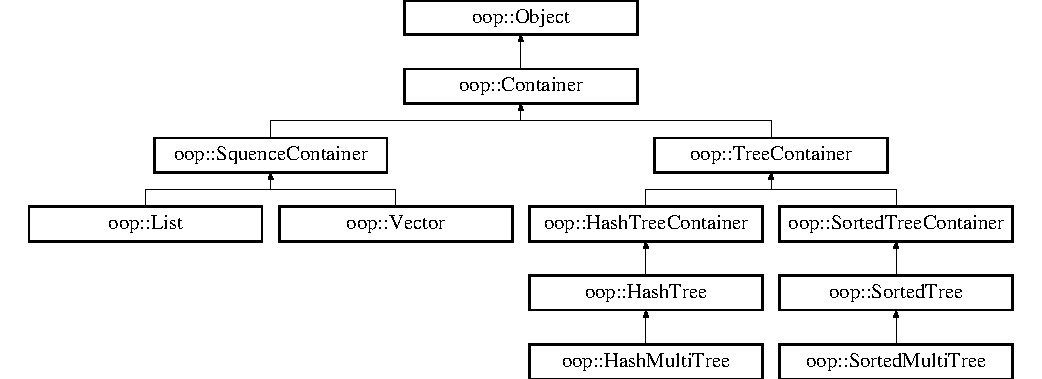
\includegraphics[height=5.090909cm]{classoop_1_1Container}
\end{center}
\end{figure}
\subsection*{\-Public \-Member \-Functions}
\begin{DoxyCompactItemize}
\item 
\hypertarget{classoop_1_1Container_ad801eba9a4943417407b6a21061517e5}{virtual int {\bfseries size} ()}\label{classoop_1_1Container_ad801eba9a4943417407b6a21061517e5}

\item 
\hypertarget{classoop_1_1Container_a8bf226d4b09f15b8c13b23de7c9cb64b}{virtual int {\bfseries empty} ()}\label{classoop_1_1Container_a8bf226d4b09f15b8c13b23de7c9cb64b}

\item 
\hypertarget{classoop_1_1Container_a4786051f94579ede522a4c81b82d6b95}{virtual void {\bfseries insert} (\hyperlink{classoop_1_1Object}{\-Object} $\ast$)}\label{classoop_1_1Container_a4786051f94579ede522a4c81b82d6b95}

\end{DoxyCompactItemize}


\subsection{\-Detailed \-Description}
klasa container dziedziczy po głównym przodku ponieważ każdy kontener jest rozserzonym obiektem 

\-The documentation for this class was generated from the following files\-:\begin{DoxyCompactItemize}
\item 
\-Container.\-h\item 
\-Container.\-cpp\end{DoxyCompactItemize}

\hypertarget{classoop_1_1HashMultiTree}{\section{oop\-:\-:\-Hash\-Multi\-Tree \-Class \-Reference}
\label{classoop_1_1HashMultiTree}\index{oop\-::\-Hash\-Multi\-Tree@{oop\-::\-Hash\-Multi\-Tree}}
}
\-Inheritance diagram for oop\-:\-:\-Hash\-Multi\-Tree\-:\begin{figure}[H]
\begin{center}
\leavevmode
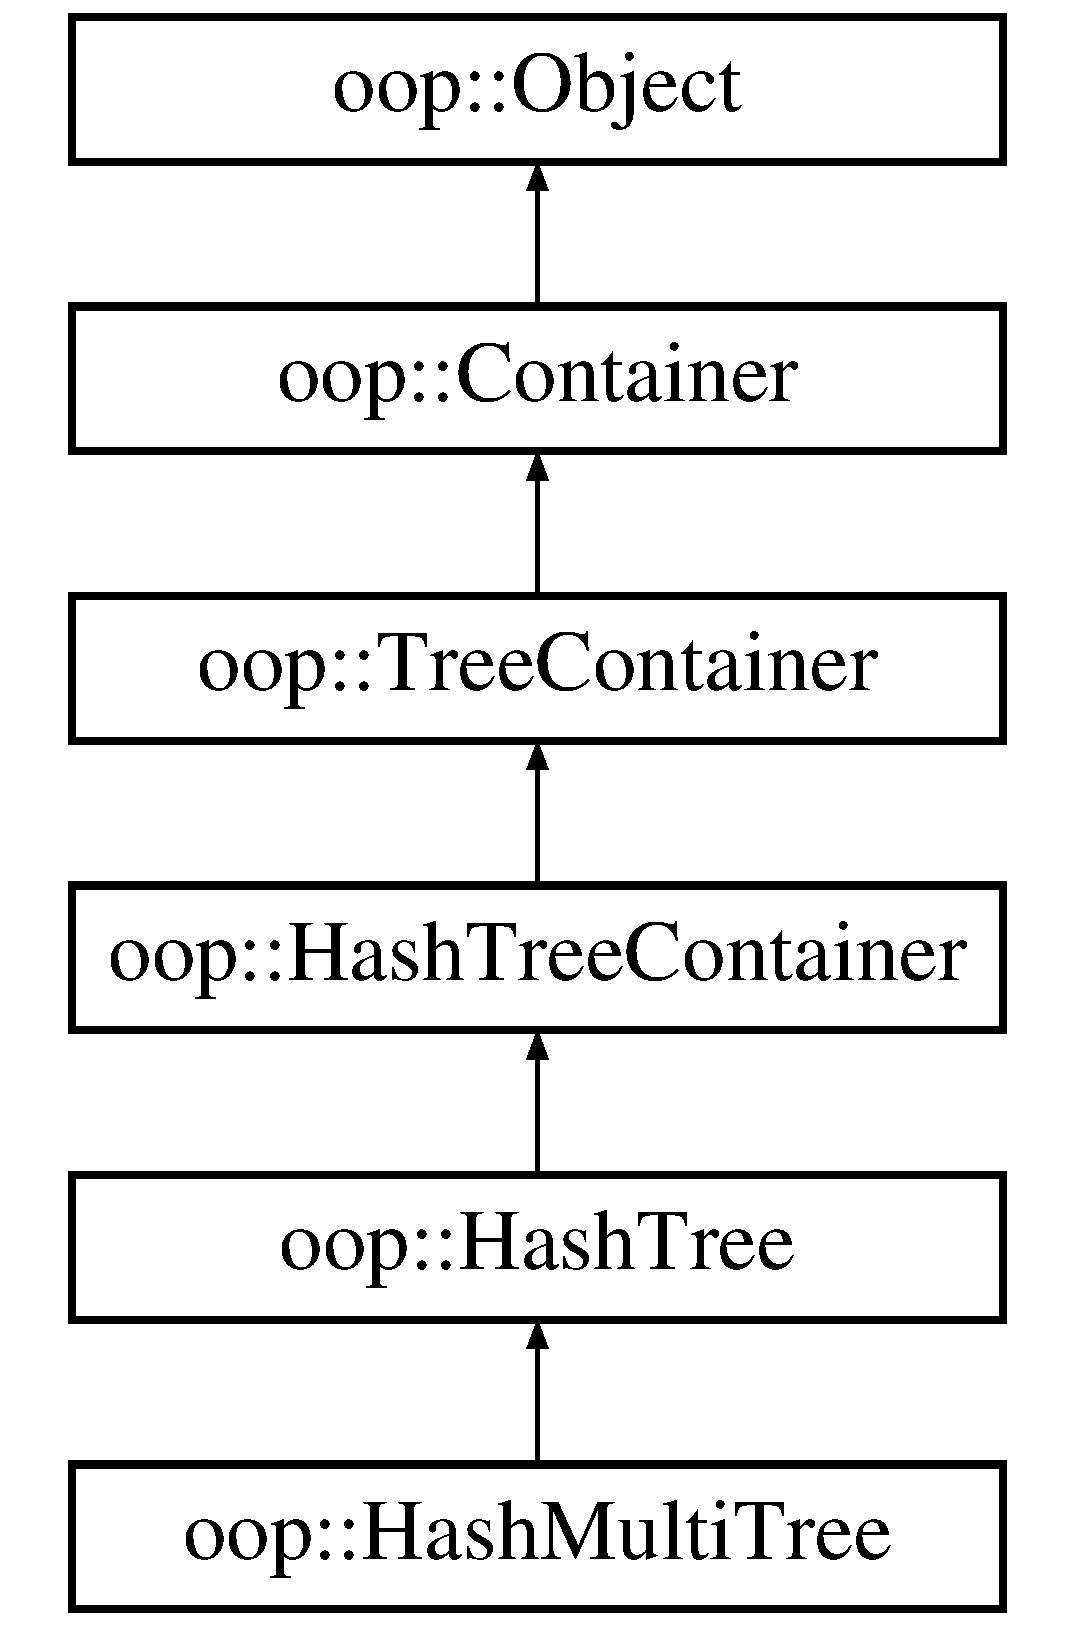
\includegraphics[height=6.000000cm]{classoop_1_1HashMultiTree}
\end{center}
\end{figure}


\-The documentation for this class was generated from the following files\-:\begin{DoxyCompactItemize}
\item 
\-Hash\-Multi\-Tree.\-h\item 
\-Hash\-Multi\-Tree.\-cpp\end{DoxyCompactItemize}

\hypertarget{classoop_1_1HashTree}{\section{oop\-:\-:\-Hash\-Tree \-Class \-Reference}
\label{classoop_1_1HashTree}\index{oop\-::\-Hash\-Tree@{oop\-::\-Hash\-Tree}}
}
\-Inheritance diagram for oop\-:\-:\-Hash\-Tree\-:\begin{figure}[H]
\begin{center}
\leavevmode
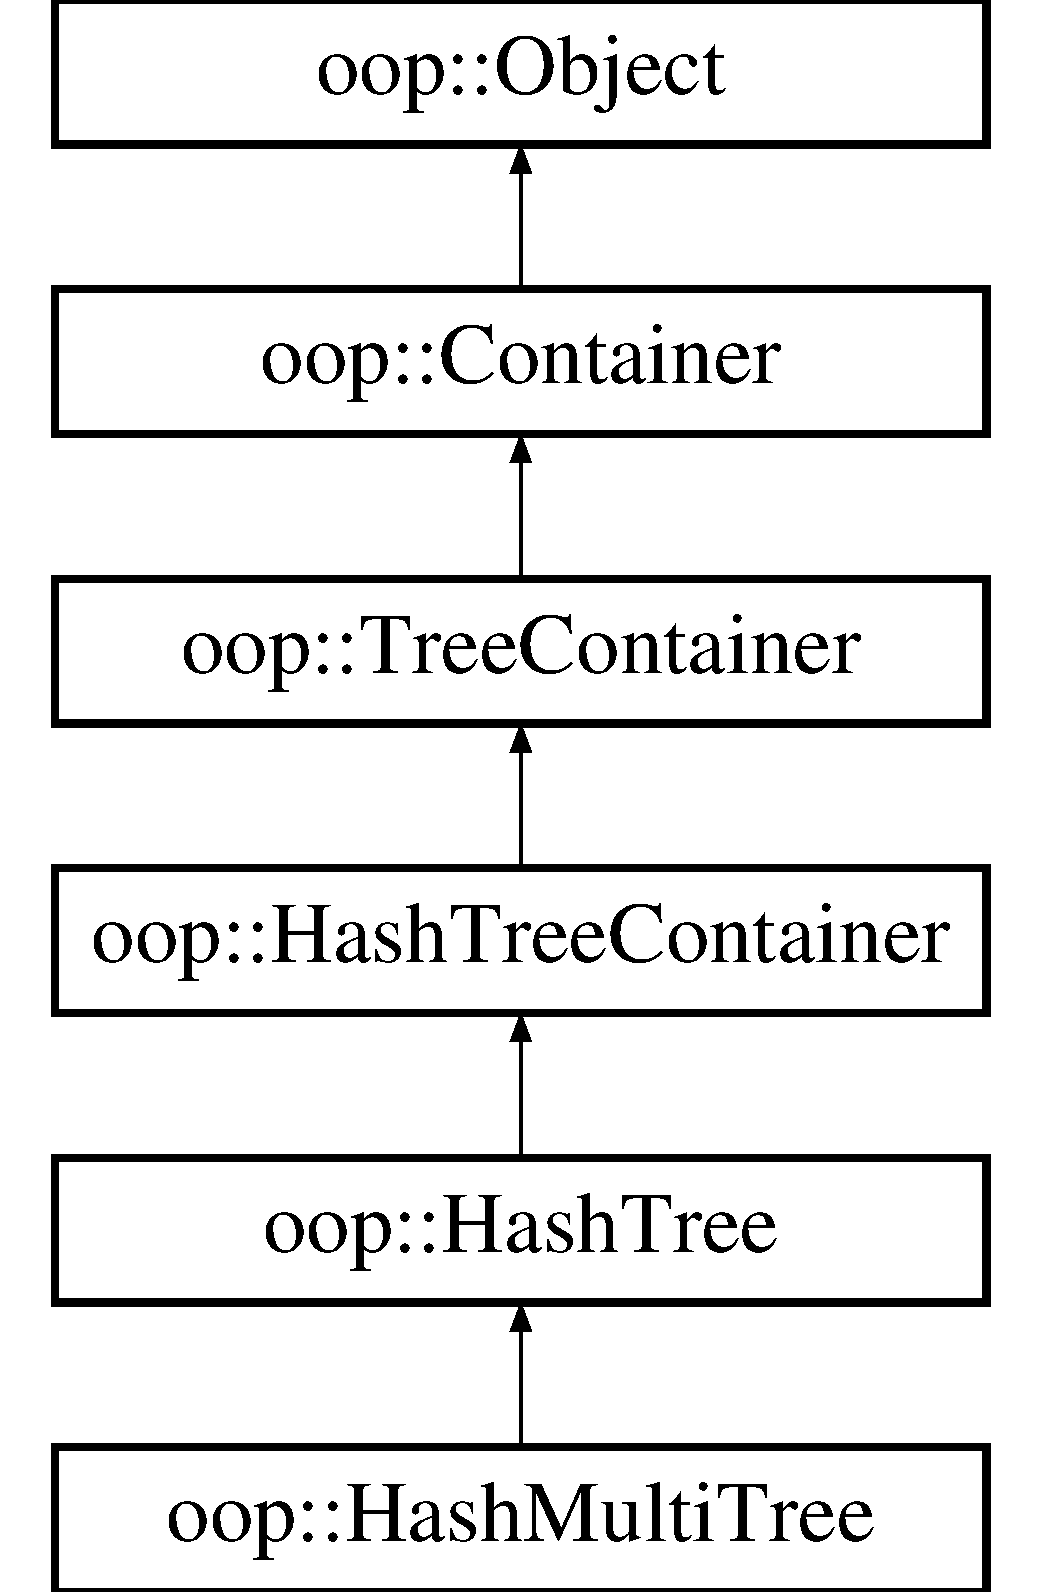
\includegraphics[height=6.000000cm]{classoop_1_1HashTree}
\end{center}
\end{figure}


\-The documentation for this class was generated from the following files\-:\begin{DoxyCompactItemize}
\item 
\-Hash\-Tree.\-h\item 
\-Hash\-Tree.\-cpp\end{DoxyCompactItemize}

\hypertarget{classoop_1_1HashTreeContainer}{\section{oop\-:\-:\-Hash\-Tree\-Container \-Class \-Reference}
\label{classoop_1_1HashTreeContainer}\index{oop\-::\-Hash\-Tree\-Container@{oop\-::\-Hash\-Tree\-Container}}
}
\-Inheritance diagram for oop\-:\-:\-Hash\-Tree\-Container\-:\begin{figure}[H]
\begin{center}
\leavevmode
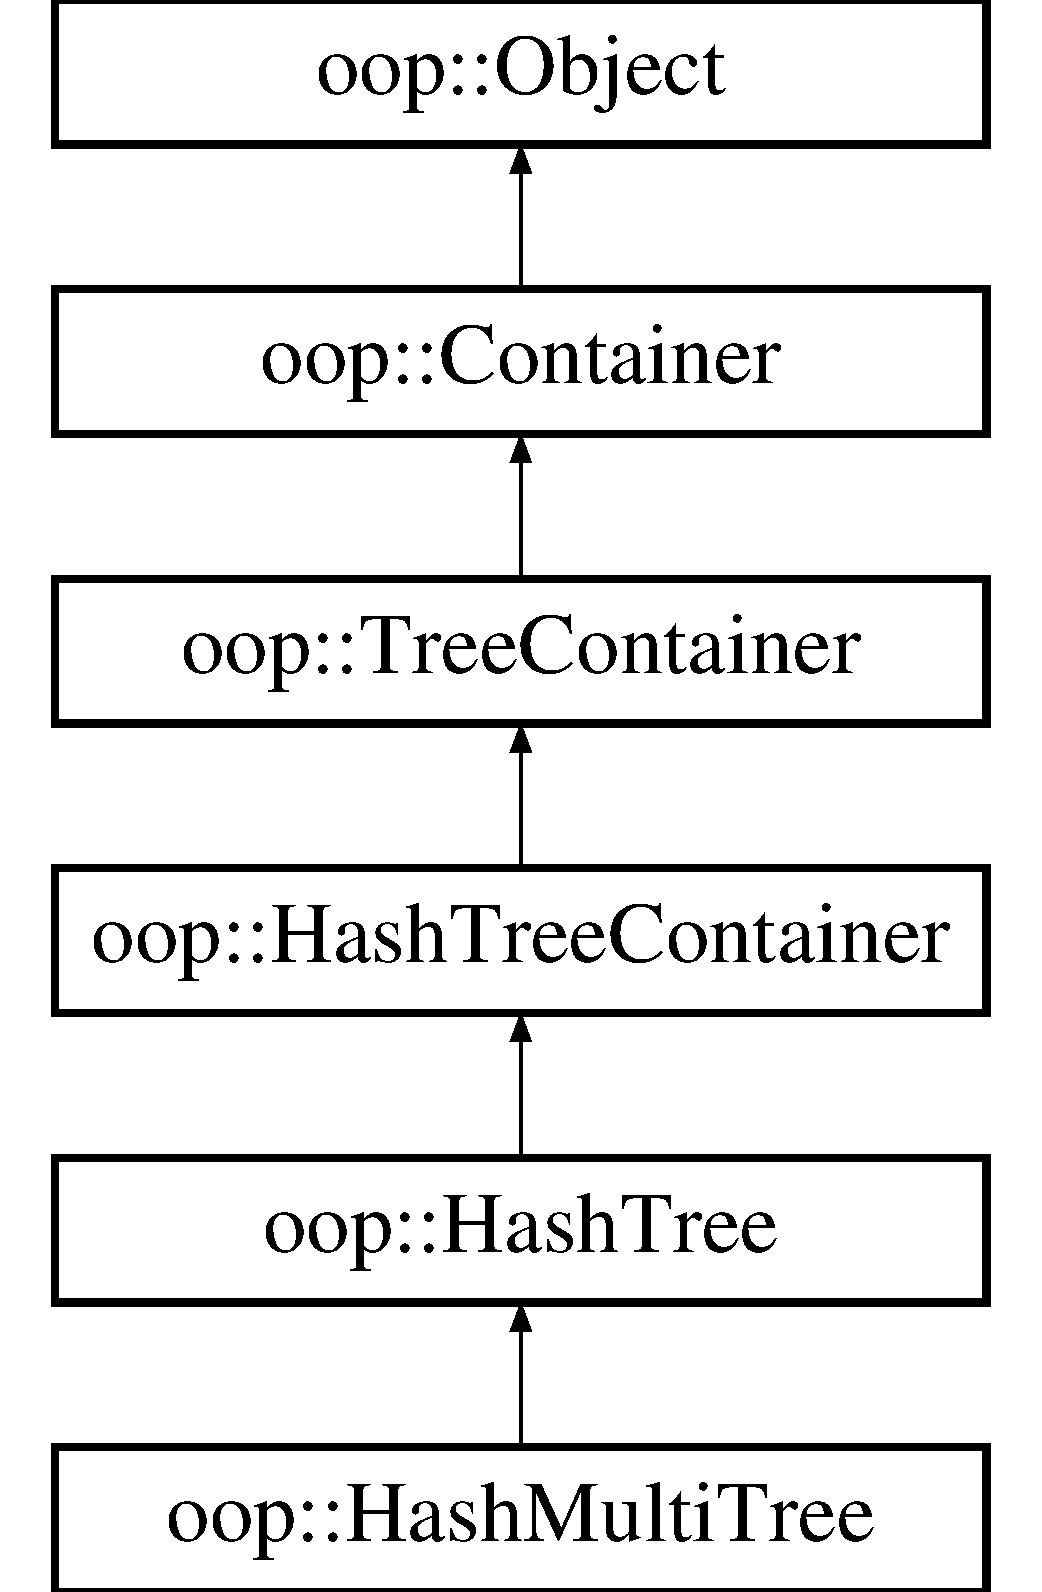
\includegraphics[height=6.000000cm]{classoop_1_1HashTreeContainer}
\end{center}
\end{figure}


\-The documentation for this class was generated from the following files\-:\begin{DoxyCompactItemize}
\item 
\-Hash\-Tree\-Container.\-h\item 
\-Hash\-Tree\-Container.\-cpp\end{DoxyCompactItemize}

\hypertarget{classoop_1_1List}{\section{oop\-:\-:\-List \-Class \-Reference}
\label{classoop_1_1List}\index{oop\-::\-List@{oop\-::\-List}}
}
\-Inheritance diagram for oop\-:\-:\-List\-:\begin{figure}[H]
\begin{center}
\leavevmode
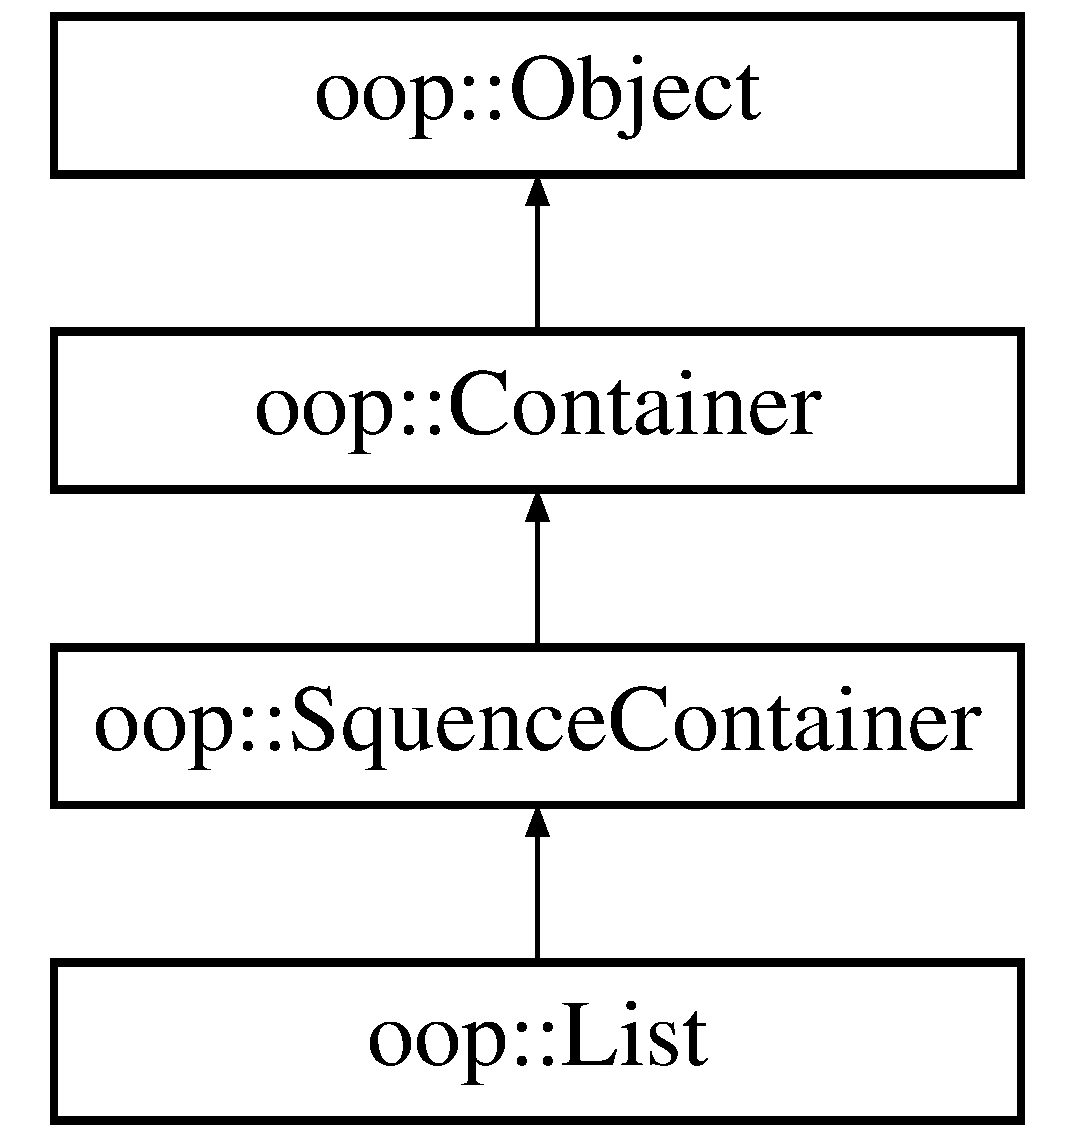
\includegraphics[height=4.000000cm]{classoop_1_1List}
\end{center}
\end{figure}


\-The documentation for this class was generated from the following files\-:\begin{DoxyCompactItemize}
\item 
\-List.\-h\item 
\-List.\-cpp\end{DoxyCompactItemize}

\hypertarget{classoop_1_1Object}{\section{oop\-:\-:\-Object \-Class \-Reference}
\label{classoop_1_1Object}\index{oop\-::\-Object@{oop\-::\-Object}}
}


{\ttfamily \#include $<$\-Object.\-h$>$}

\-Inheritance diagram for oop\-:\-:\-Object\-:\begin{figure}[H]
\begin{center}
\leavevmode
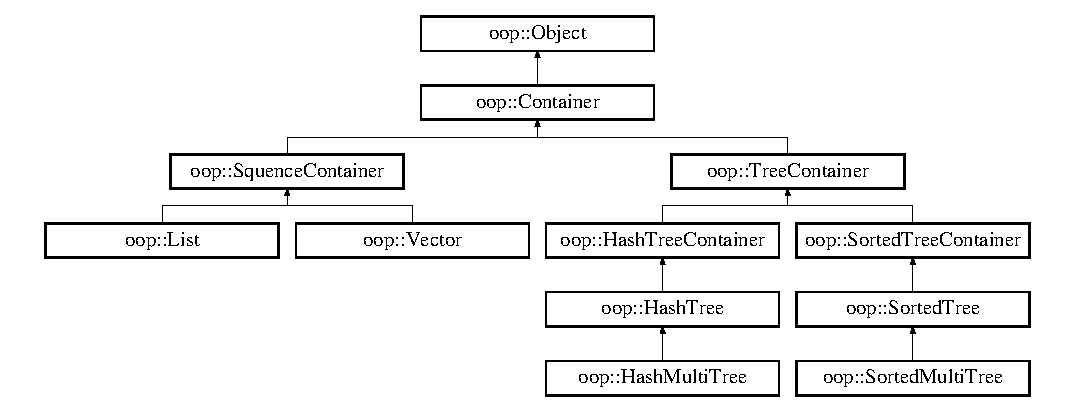
\includegraphics[height=5.090909cm]{classoop_1_1Object}
\end{center}
\end{figure}
\subsection*{\-Public \-Member \-Functions}
\begin{DoxyCompactItemize}
\item 
\hypertarget{classoop_1_1Object_a0120a77777b44355aa7f1d8b4bf43954}{virtual std\-::string {\bfseries name} ()}\label{classoop_1_1Object_a0120a77777b44355aa7f1d8b4bf43954}

\end{DoxyCompactItemize}


\subsection{\-Detailed \-Description}
\-Główny obiekt przodek 

\-The documentation for this class was generated from the following files\-:\begin{DoxyCompactItemize}
\item 
\-Object.\-h\item 
\-Object.\-cpp\end{DoxyCompactItemize}

\hypertarget{classoop_1_1SortedMultiTree}{\section{oop\-:\-:\-Sorted\-Multi\-Tree \-Class \-Reference}
\label{classoop_1_1SortedMultiTree}\index{oop\-::\-Sorted\-Multi\-Tree@{oop\-::\-Sorted\-Multi\-Tree}}
}
\-Inheritance diagram for oop\-:\-:\-Sorted\-Multi\-Tree\-:\begin{figure}[H]
\begin{center}
\leavevmode
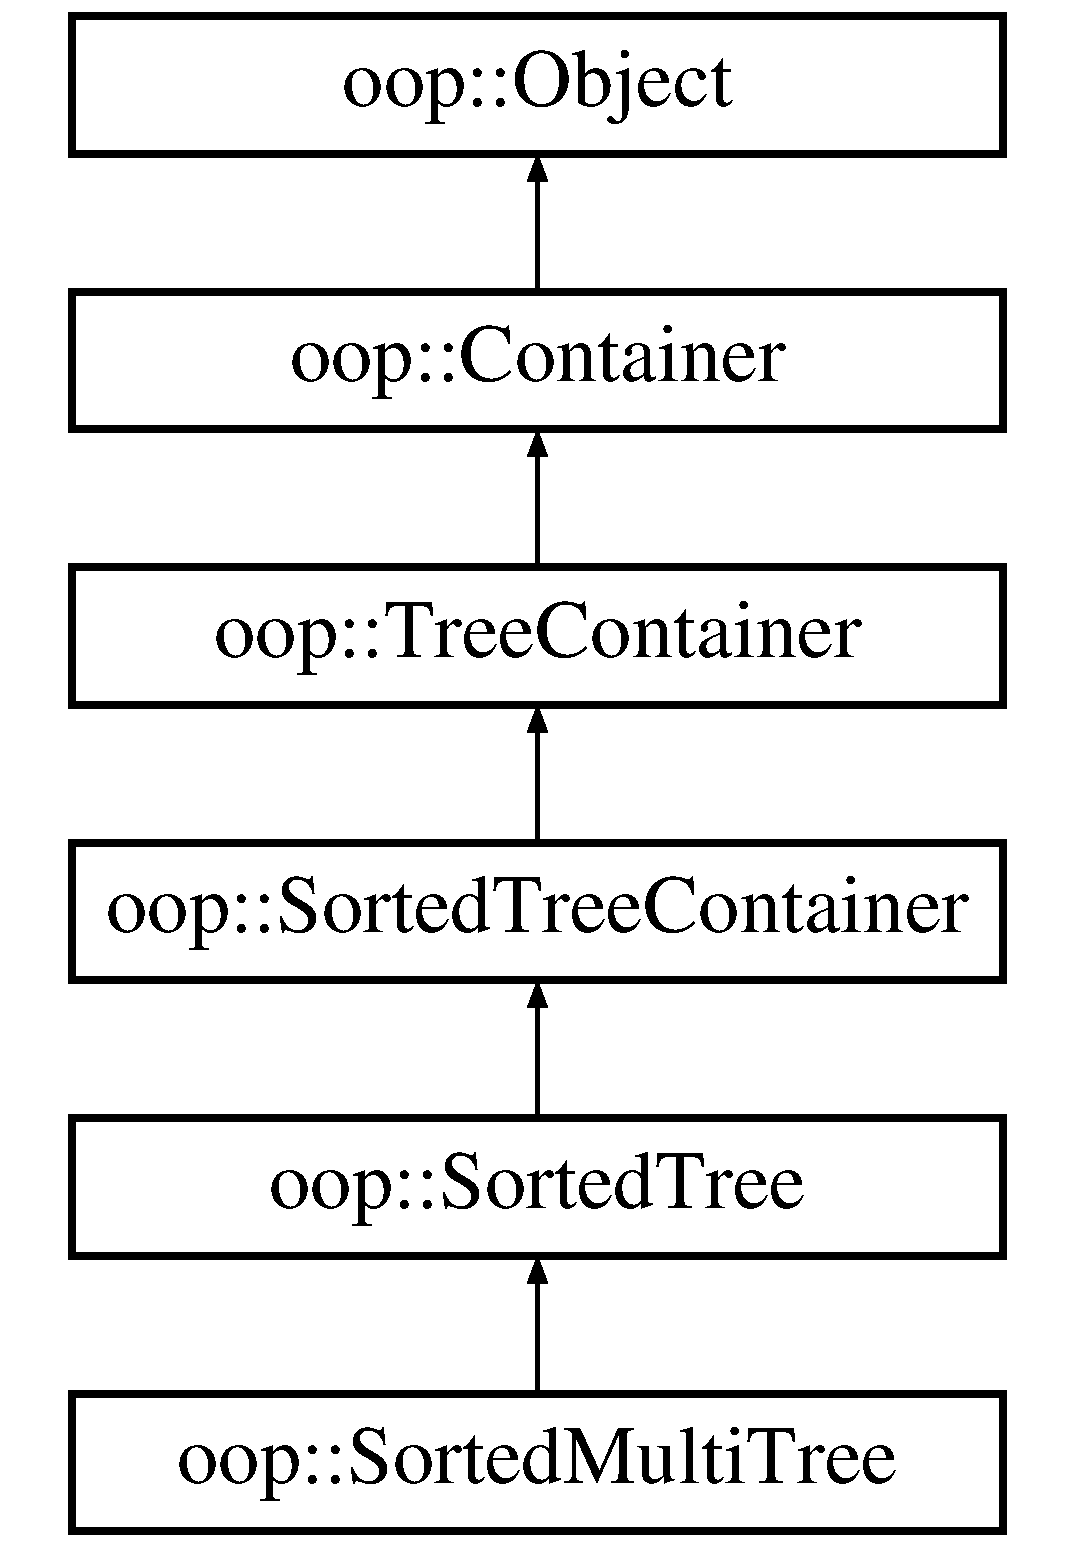
\includegraphics[height=6.000000cm]{classoop_1_1SortedMultiTree}
\end{center}
\end{figure}


\-The documentation for this class was generated from the following files\-:\begin{DoxyCompactItemize}
\item 
\-Sorted\-Multi\-Tree.\-h\item 
\-Sorted\-Multi\-Tree.\-cpp\end{DoxyCompactItemize}

\hypertarget{classoop_1_1SortedTree}{\section{oop\-:\-:\-Sorted\-Tree \-Class \-Reference}
\label{classoop_1_1SortedTree}\index{oop\-::\-Sorted\-Tree@{oop\-::\-Sorted\-Tree}}
}
\-Inheritance diagram for oop\-:\-:\-Sorted\-Tree\-:\begin{figure}[H]
\begin{center}
\leavevmode
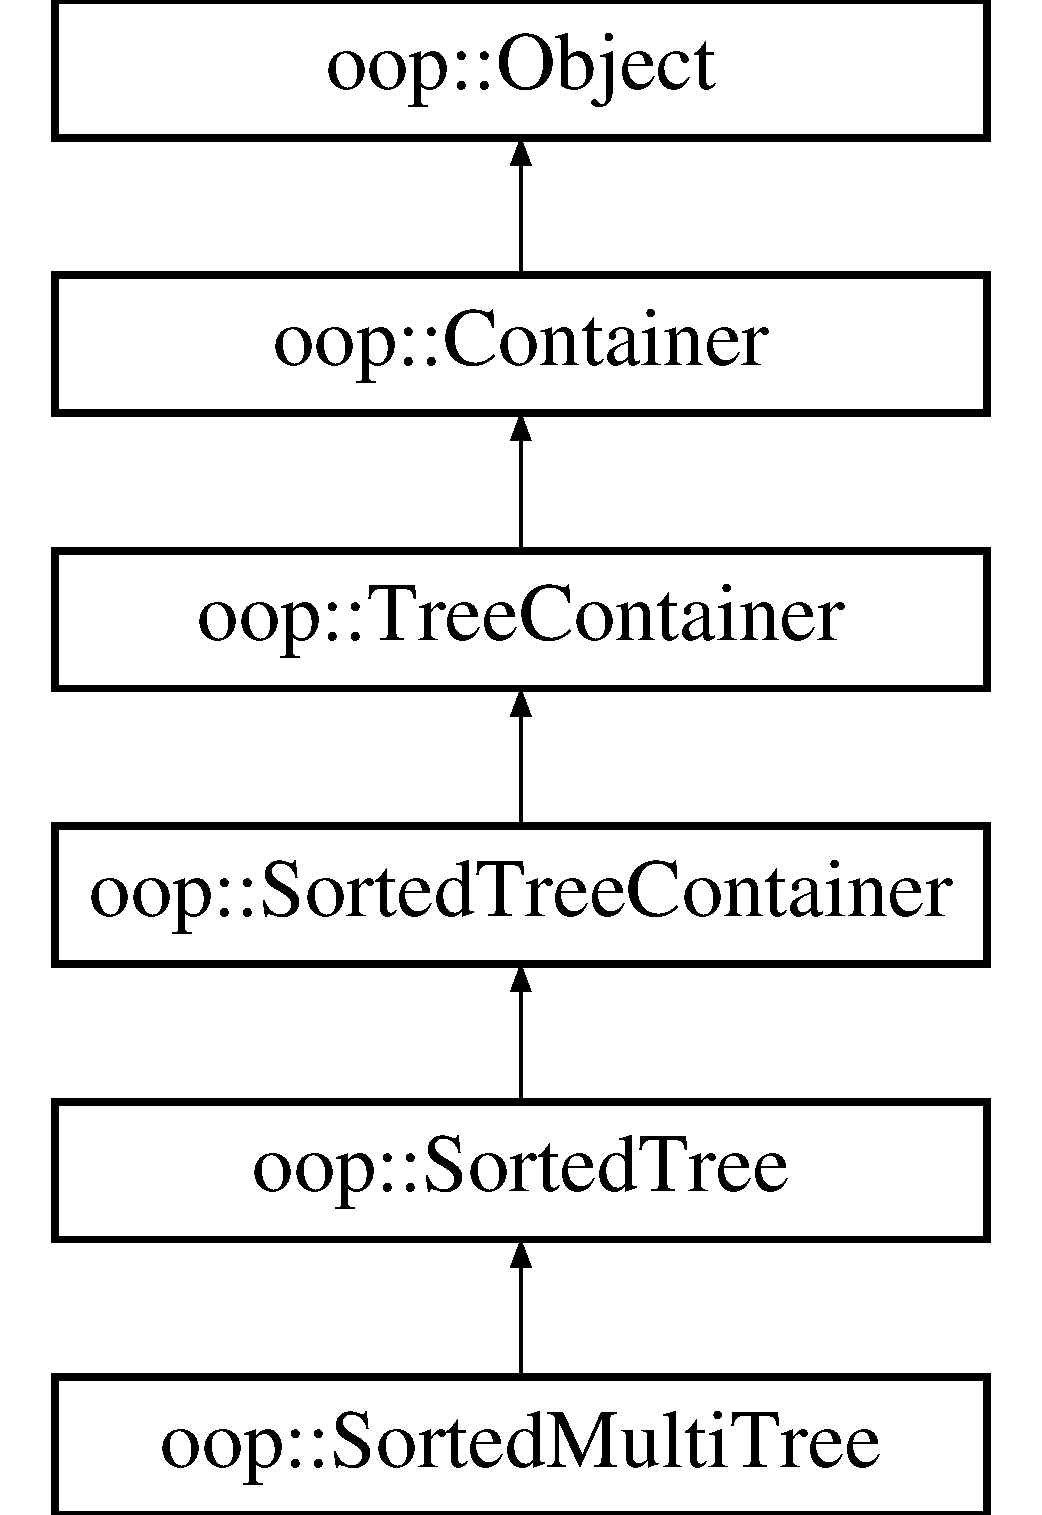
\includegraphics[height=6.000000cm]{classoop_1_1SortedTree}
\end{center}
\end{figure}


\-The documentation for this class was generated from the following files\-:\begin{DoxyCompactItemize}
\item 
\-Sorted\-Tree.\-h\item 
\-Sorted\-Tree.\-cpp\end{DoxyCompactItemize}

\hypertarget{classoop_1_1SortedTreeContainer}{\section{oop\-:\-:\-Sorted\-Tree\-Container \-Class \-Reference}
\label{classoop_1_1SortedTreeContainer}\index{oop\-::\-Sorted\-Tree\-Container@{oop\-::\-Sorted\-Tree\-Container}}
}
\-Inheritance diagram for oop\-:\-:\-Sorted\-Tree\-Container\-:\begin{figure}[H]
\begin{center}
\leavevmode
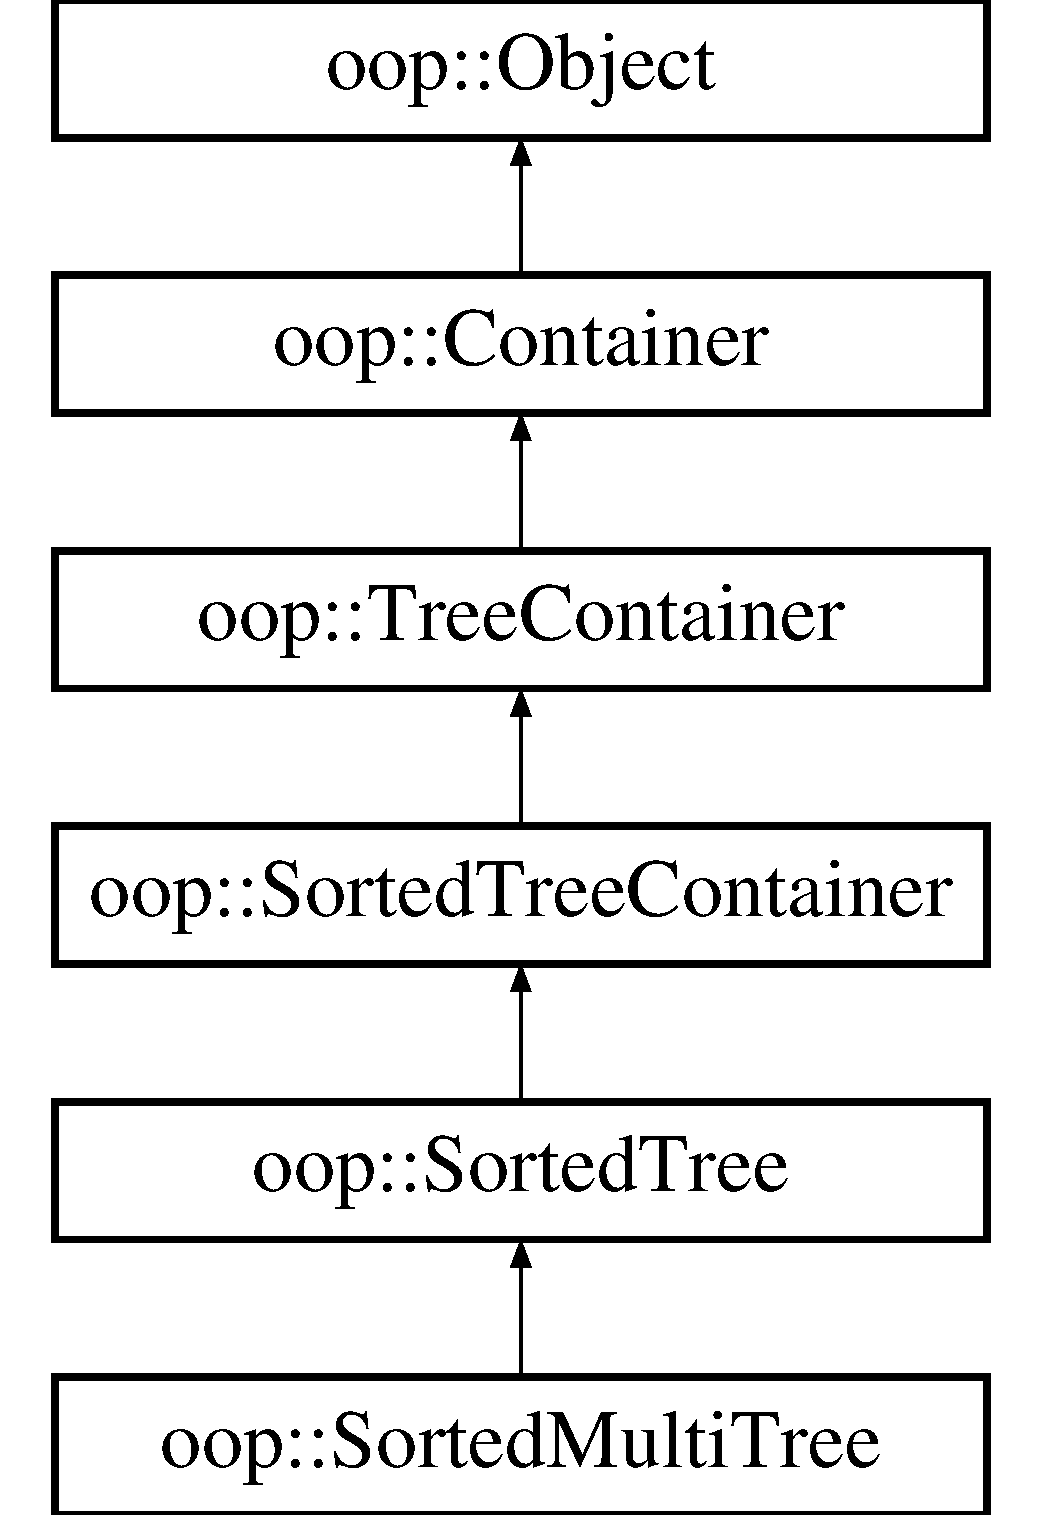
\includegraphics[height=6.000000cm]{classoop_1_1SortedTreeContainer}
\end{center}
\end{figure}


\-The documentation for this class was generated from the following files\-:\begin{DoxyCompactItemize}
\item 
\-Sorted\-Tree\-Container.\-h\item 
\-Sorted\-Tree\-Container.\-cpp\end{DoxyCompactItemize}

\hypertarget{classoop_1_1SquenceContainer}{\section{oop\-:\-:\-Squence\-Container \-Class \-Reference}
\label{classoop_1_1SquenceContainer}\index{oop\-::\-Squence\-Container@{oop\-::\-Squence\-Container}}
}


{\ttfamily \#include $<$\-Squence\-Container.\-h$>$}

\-Inheritance diagram for oop\-:\-:\-Squence\-Container\-:\begin{figure}[H]
\begin{center}
\leavevmode
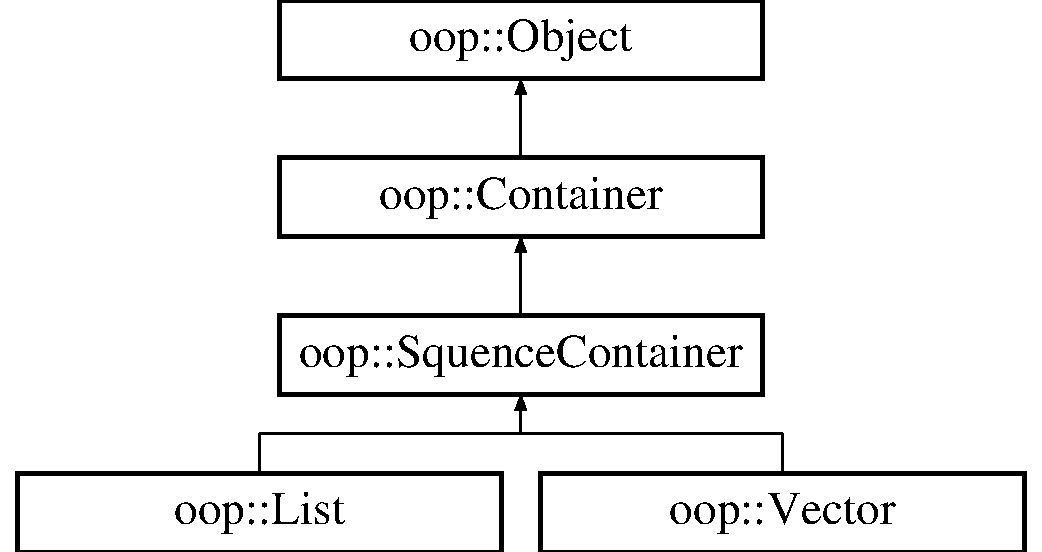
\includegraphics[height=4.000000cm]{classoop_1_1SquenceContainer}
\end{center}
\end{figure}
\subsection*{\-Public \-Member \-Functions}
\begin{DoxyCompactItemize}
\item 
\hypertarget{classoop_1_1SquenceContainer_a2106fdced5444a932f21a7400a864a3c}{virtual void {\bfseries push\-\_\-back} (\hyperlink{classoop_1_1Object}{\-Object} $\ast$)}\label{classoop_1_1SquenceContainer_a2106fdced5444a932f21a7400a864a3c}

\item 
\hypertarget{classoop_1_1SquenceContainer_ae40b6c7f54dbf7568f16cec7d2f11b6c}{virtual void {\bfseries push\-\_\-front} (\hyperlink{classoop_1_1Object}{\-Object} $\ast$)}\label{classoop_1_1SquenceContainer_ae40b6c7f54dbf7568f16cec7d2f11b6c}

\end{DoxyCompactItemize}


\subsection{\-Detailed \-Description}
\hyperlink{classoop_1_1SquenceContainer}{\-Squence\-Container} dziedziczy po \hyperlink{classoop_1_1Container}{\-Container} ponieważ jest to pojemnik w którym dane mają swoja kolejność 

\-The documentation for this class was generated from the following files\-:\begin{DoxyCompactItemize}
\item 
\-Squence\-Container.\-h\item 
\-Squence\-Container.\-cpp\end{DoxyCompactItemize}

\hypertarget{structtool}{\section{tool \-Struct \-Reference}
\label{structtool}\index{tool@{tool}}
}
\subsection*{\-Static \-Public \-Member \-Functions}
\begin{DoxyCompactItemize}
\item 
\hypertarget{structtool_a4d7c73cebcdb1f0ed2d1441f6bdeed24}{static std\-::string {\bfseries rtti\-\_\-real\-\_\-name} (const char $\ast$name)}\label{structtool_a4d7c73cebcdb1f0ed2d1441f6bdeed24}

\end{DoxyCompactItemize}


\-The documentation for this struct was generated from the following file\-:\begin{DoxyCompactItemize}
\item 
main.\-cpp\end{DoxyCompactItemize}

\hypertarget{classoop_1_1TreeContainer}{\section{oop\-:\-:\-Tree\-Container \-Class \-Reference}
\label{classoop_1_1TreeContainer}\index{oop\-::\-Tree\-Container@{oop\-::\-Tree\-Container}}
}


{\ttfamily \#include $<$\-Tree\-Container.\-h$>$}

\-Inheritance diagram for oop\-:\-:\-Tree\-Container\-:\begin{figure}[H]
\begin{center}
\leavevmode
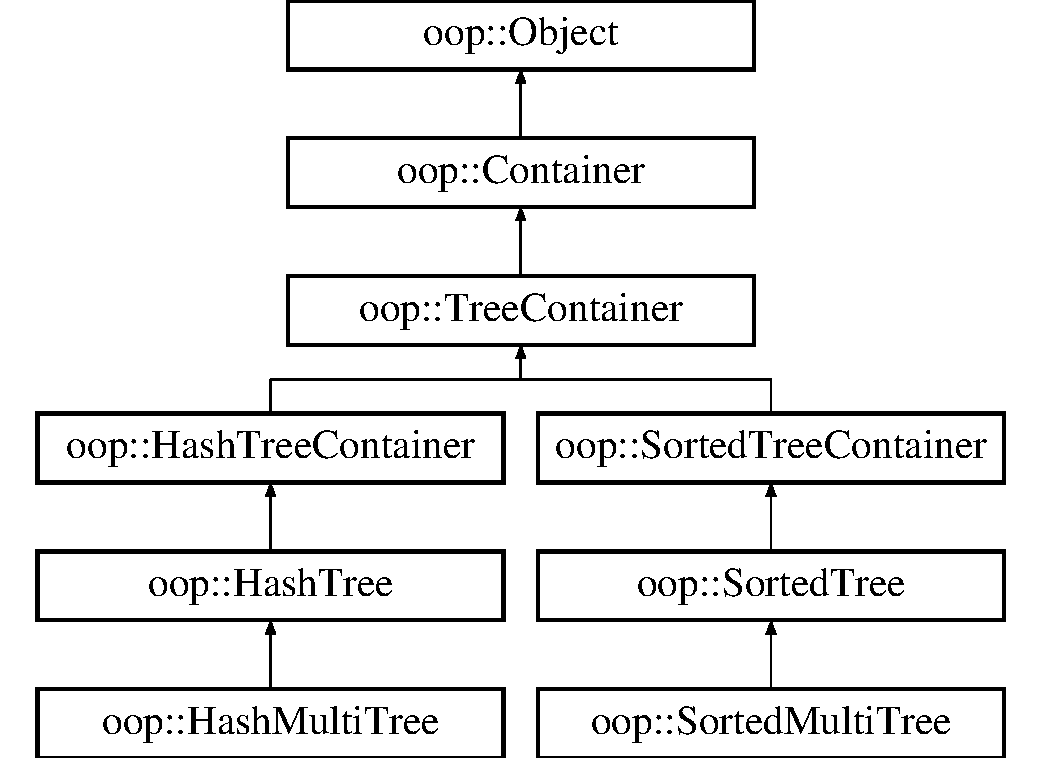
\includegraphics[height=6.000000cm]{classoop_1_1TreeContainer}
\end{center}
\end{figure}


\subsection{\-Detailed \-Description}
\-Klasa dziedziczy po \hyperlink{classoop_1_1Container}{\-Container} ponieważ dane są ustawione jak drzewo 

\-The documentation for this class was generated from the following files\-:\begin{DoxyCompactItemize}
\item 
\-Tree\-Container.\-h\item 
\-Tree\-Container.\-cpp\end{DoxyCompactItemize}

\hypertarget{classoop_1_1Vector}{\section{oop\-:\-:\-Vector \-Class \-Reference}
\label{classoop_1_1Vector}\index{oop\-::\-Vector@{oop\-::\-Vector}}
}
\-Inheritance diagram for oop\-:\-:\-Vector\-:\begin{figure}[H]
\begin{center}
\leavevmode
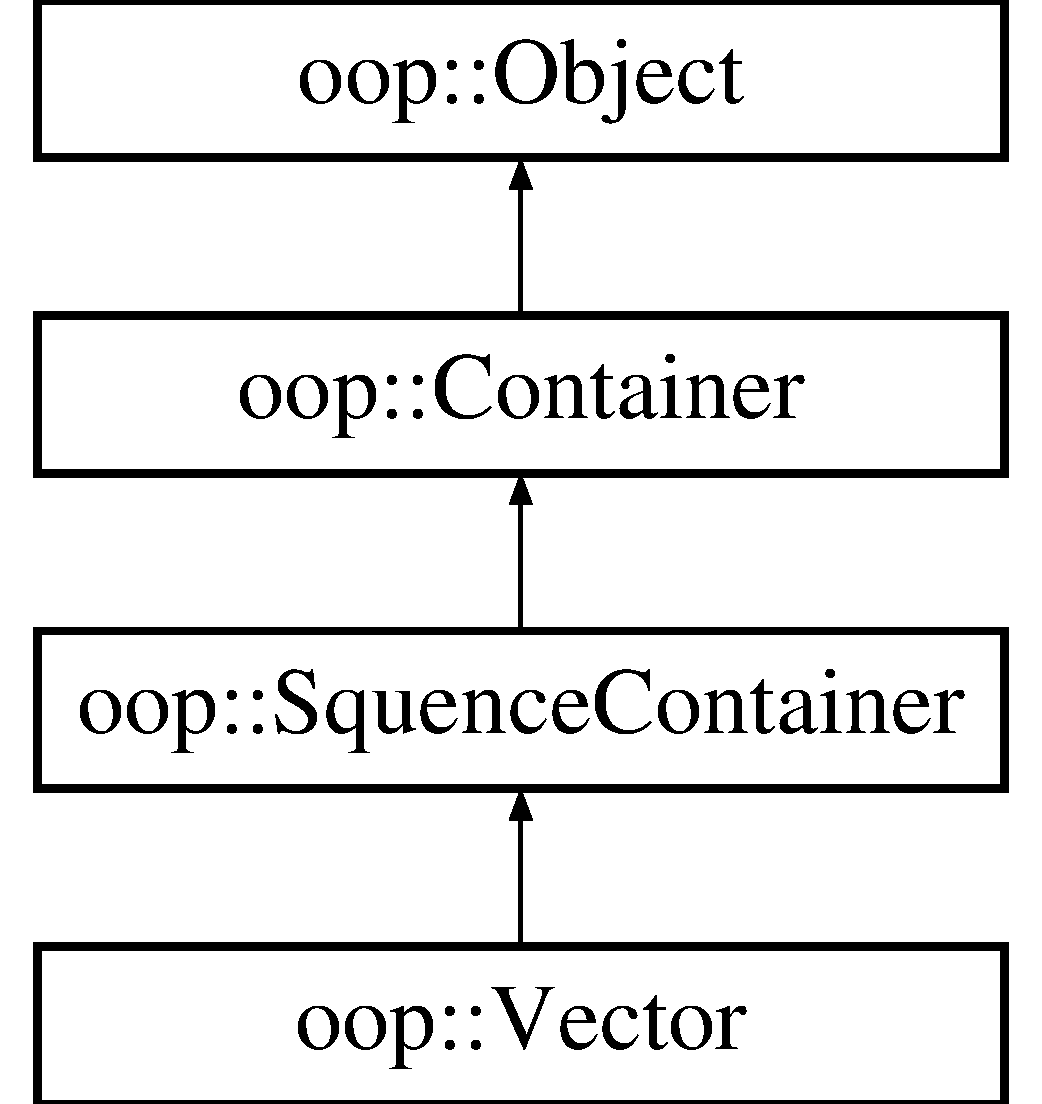
\includegraphics[height=4.000000cm]{classoop_1_1Vector}
\end{center}
\end{figure}


\-The documentation for this class was generated from the following files\-:\begin{DoxyCompactItemize}
\item 
\-Vector.\-h\item 
\-Vector.\-cpp\end{DoxyCompactItemize}

\printindex
\end{document}
